%!TEX root = ../thesis.tex

\section{実験概要}
本章では, 前章の実験で使用した教師データに問題があるか調査するために, 2種類の実験を行う. 1つ目は教師データを入れ替えた実験, 2つ目はカメラを9個にした実験である. これらの実験により, 目標角速度とカメラ画像に問題があるかを明らかにする. 

\section{実験方法}
まず初めに, 教師データを入れ替えた実験に関して説明する. \figref{Fig:change}のように, 5章で最も成功率の高かった実験(以後, 実験1と呼ぶ)で使用した教師データと, 前章の実験(以後, 実験2と呼ぶ)で使用した教師データを入れ替えて学習を行う.
\par 次に, カメラを9個にした実験について説明する. カメラの取り付け位置は, 前章の3つのカメラそれぞれを基準として, ヨー方向に±5[deg]回転させたカメラを追加する. このロボットを使用して, 走行させながらデータ収集を行う. 目標角速度に関しては, 前章のオフセットを用いる. 
\par 原因の調査を行うために, シミュレータを用いた実験を行う. 実験環境, 実験装置は前章と同様のシミュレータ環境を用いる.また, 学習器の訓練条件, 学習したモデルを用いたテストなどの条件は前章と同様とする. 実験1の目標角速度と実験2のカメラ画像の組み合わせを実験3, 実験1のカメラ画像と実験2の目標角速度の組み合わせを実験4, カメラを9個にした実験を実験5とする. 

\begin{figure}[h]
  \centering
  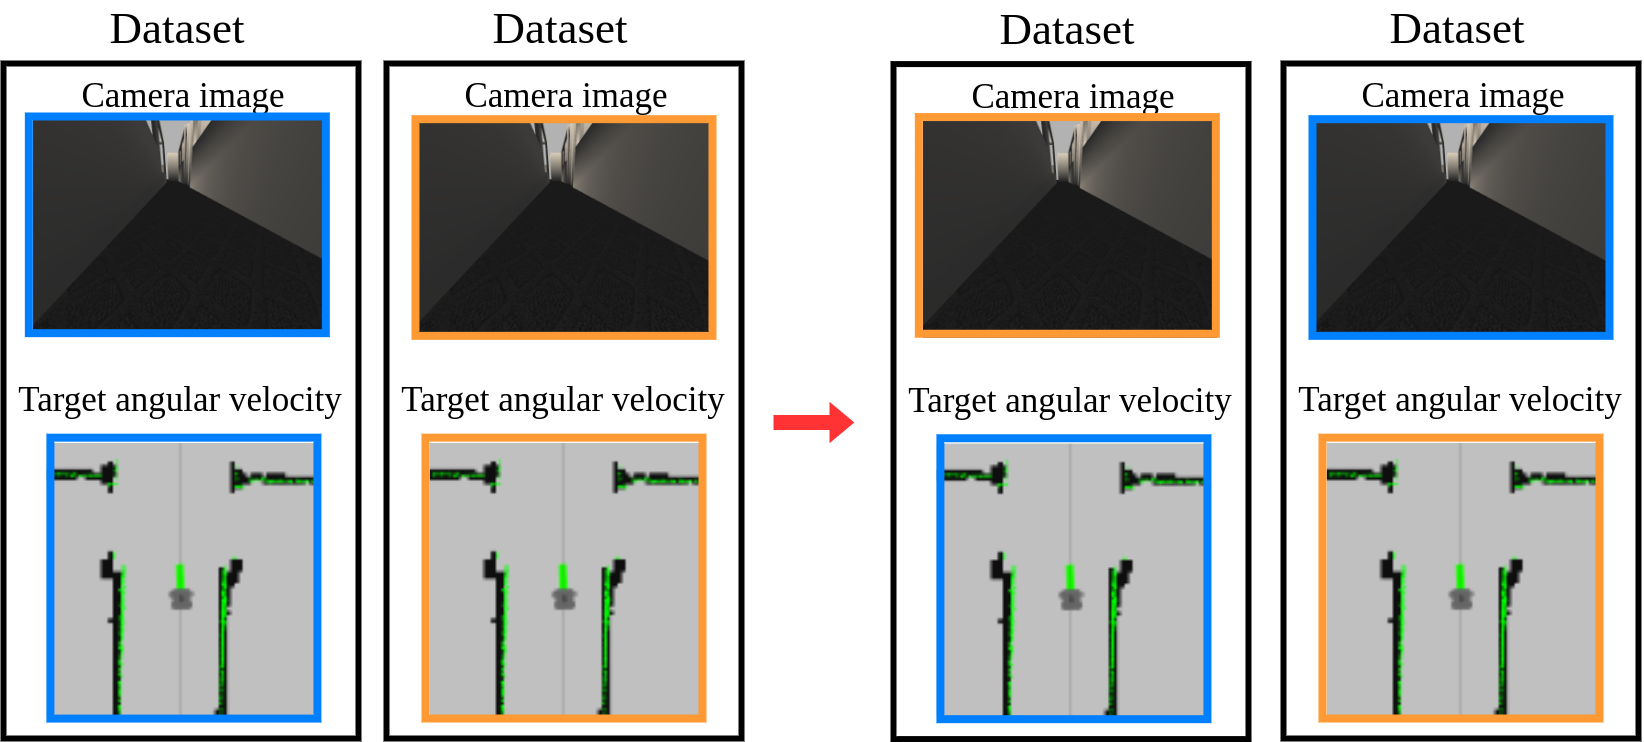
\includegraphics[keepaspectratio, scale=0.22]{images/change.png}
  \caption{Exchange of supervisory data}
  \label{Fig:change}
\end{figure}

\newpage
\subsection{実験結果と考察}
実験結果を\ref{tb:inves}に示す. 分母の30は実験回数を示しており, 分子の数は成功回数を示している. 結果的に, 実験3, 実験4, 実験5の成功回数はいずれも30回中0回となった. 失敗した箇所も, 概ね実験2と同様に, 直進時に目標経路から外れて, 壁に衝突して失敗した. \figref{Fig:sample3}, \figref{Fig:sample4}, \figref{Fig:sample5}, に, 実験3, 実験4, 実験5それぞれの条件で学習した際のlossのグラフを示す. lossの値からも正しく学習できないと考えられる. 
\par これらのことから, カメラ画像から左右に切り抜く方法では, ロボットをヨー方向に±5[deg]回転させた際の画像を再現できていないと考えられる. また, 目標角速度に関しても, 実験1ではそれぞれの位置と向きでルールベース制御器の出力を取得していた. しかし, 実験2ではロボットを走行させながら収集した角速度に, オフセットを加えることで, 各位置と向きを考慮した目標角速度を生成している. この方法では, 経路追従を継続するのに必要な目標角速度を再現できていないと考えられる. オフセットの値に関しても, 値が大きいあるいは小さいために, 目標経路から外れたり, 復帰することができていないと考えられる. 目標経路及び±0.2の位置, 0[deg]及び±5[deg]の向きに, ロボットを配置した際に得られるカメラ画像と目標角速度を, どのように再現するかは今後の課題としたい. 

\newpage
\begin{table}[h]
  \centering
  \caption{Number of successes in the experiments of simulator}
  \begin{tabular}{|c|c|} \hline
      Experiments & Number of successes \\ \hline
      Exp. 3 & 0/30 \\ \hline
      Exp. 4 & 0/30 \\ \hline
      Exp. 5 & 0/30 \\ \hline
    \end{tabular}
  \label{tb:inves}
\end{table}

\begin{figure}[h]
  \centering
  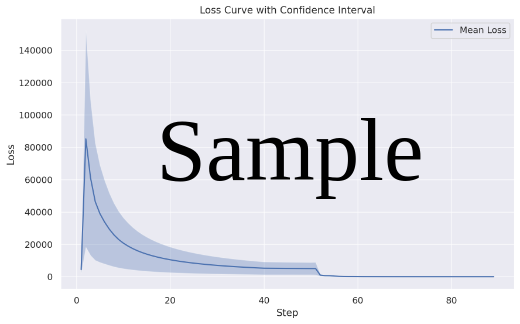
\includegraphics[keepaspectratio, scale=0.55]{images/sample.png}
  \caption{Loss value in the experiment3}
  \label{Fig:sample3}
\end{figure}

\begin{figure}[h]
  \centering
  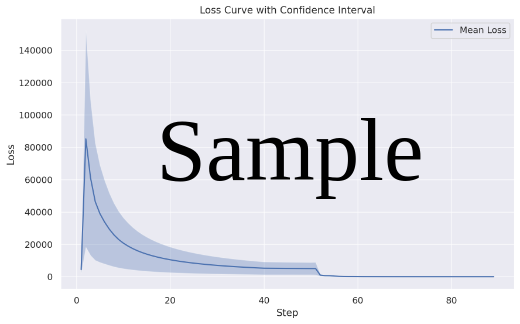
\includegraphics[keepaspectratio, scale=0.55]{images/sample.png}
  \caption{Loss value in the experiment4}
  \label{Fig:sample4}
\end{figure}

\begin{figure}[h]
  \centering
  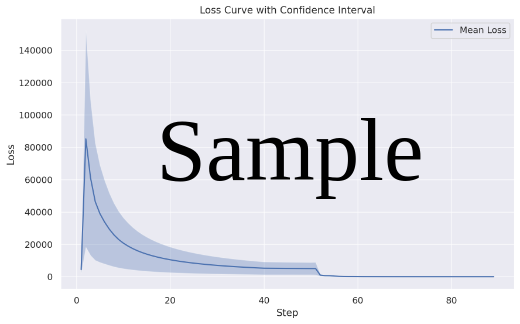
\includegraphics[keepaspectratio, scale=0.55]{images/sample.png}
  \caption{Loss value in the experiment5}
  \label{Fig:sample5}
\end{figure}

\newpage
\section{まとめ}
本章では, 前章の実験で使用した教師データに問題があるか調査を行った. シミュレータを用いた実験により, 以下のことを確認した.

\begin{itemize}
  \item 3つのカメラから得られる画像を切り抜く手法では, ロボットをヨー方向に±5[deg]回転させた際の画像を再現できていなく, 画像に問題があることを確認
  \item ロボットを走行させた際に得られる目標角速度に, オフセットを加えた値に問題があることを確認
  \item オフセットの値が大きいあるいは小さいために, 目標経路から外れたり, 復帰することができていないと考えられる.
\end{itemize}

% 前章で最も成功率の高かった際の教師データを実験1, 本章の教師データを実験2として比較を行う. これにより, 目標角速度とカメラ画像に問題があるかを調査する. \figref{Fig:ratio}に目標角速度の割合を比較したグラフを示す. 

% \begin{figure}[h]
%   \centering
%   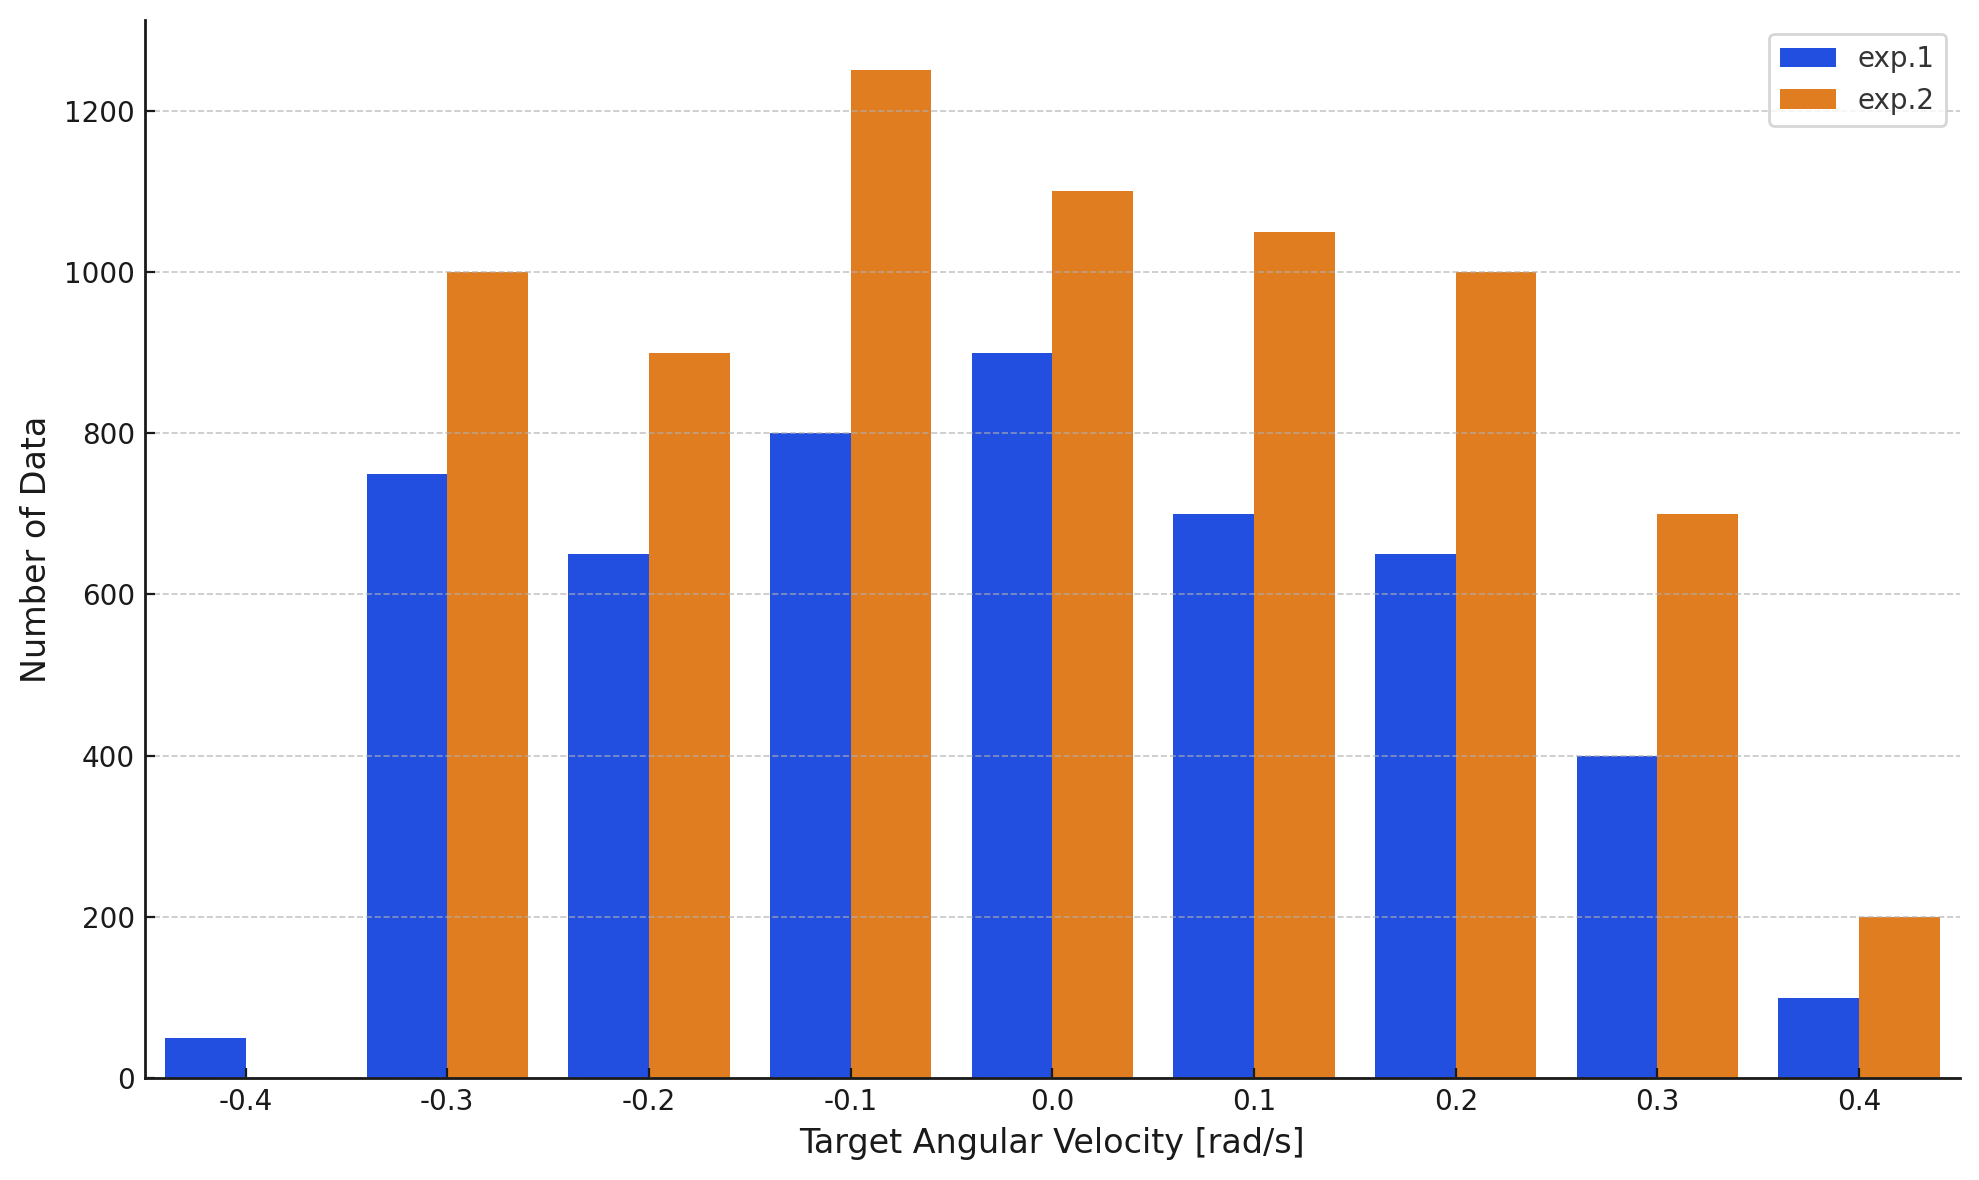
\includegraphics[keepaspectratio, scale=0.5]{images/output.png}
%   \caption{Comparison of target angular velocity ratios}
%   \label{Fig:ratio}
% \end{figure}

% 実験1と実験2の教師データを入れ替えて実験を行った. まず, 実験1のカメラ画像と実験2の目標角速度の組み合わせで学習を行った.